%% bare_conf.tex
%% V1.4b
%% 2015/08/26
%% by Michael Shell
%% See:
%% http://www.michaelshell.org/
%% for current contact information.
%% 
%% This is a skeleton file demonstrating the use of IEEEtran.cls
%% (requires IEEEtran.cls version 1.8b or later) with an IEEE
%% conference paper.
%%
%% Support sites:
%% http://www.michaelshell.org/tex/ieeetran/
%% http://www.ctan.org/pkg/ieeetran
%% and
%% http://www.ieee.org/

%%*************************************************************************
%% Legal Notice:
%% This code is offered as-is without any warranty either expressed or
%% implied; without even the implied warranty of MERCHANTABILITY or
%% FITNESS FOR A PARTICULAR PURPOSE! 
%% User assumes all risk.
%% In no event shall the IEEE or any contributor to this code be liable for
%% any damages or losses, including, but not limited to, incidental,
%% consequential, or any other damages, resulting from the use or misuse
%% of any information contained here.
%%
%% All comments are the opinions of their respective authors and are not
%% necessarily endorsed by the IEEE.
%%
%% This work is distributed under the LaTeX Project Public License (LPPL)
%% ( http://www.latex-project.org/ ) version 1.3, and may be freely used,
%% distributed and modified. A copy of the LPPL, version 1.3, is included
%% in the base LaTeX documentation of all distributions of LaTeX released
%% 2003/12/01 or later.
%% Retain all contribution notices and credits.
%% ** Modified files should be clearly indicated as such, including  **
%% ** renaming them and changing author support contact information. **
%%*************************************************************************


% *** Authors should verify (and, if needed, correct) their LaTeX system  ***
% *** with the testflow diagnostic prior to trusting their LaTeX platform ***
% *** with production work. The IEEE's font choices and paper sizes can   ***
% *** trigger bugs that do not appear when using other class files.       ***                          ***
% The testflow support page is at:
% http://www.michaelshell.org/tex/testflow/



\documentclass[conference]{IEEEtran}
% Some Computer Society conferences also require the compsoc mode option,
% but others use the standard conference format.
%
% If IEEEtran.cls has not been installed into the LaTeX system files,
% manually specify the path to it like:
% \documentclass[conference]{../sty/IEEEtran}





% Some very useful LaTeX packages include:
% (uncomment the ones you want to load)


% *** MISC UTILITY PACKAGES ***
%
%\usepackage{ifpdf}
% Heiko Oberdiek's ifpdf.sty is very useful if you need conditional
% compilation based on whether the output is pdf or dvi.
% usage:
% \ifpdf
%   % pdf code
% \else
%   % dvi code
% \fi
% The latest version of ifpdf.sty can be obtained from:
% http://www.ctan.org/pkg/ifpdf
% Also, note that IEEEtran.cls V1.7 and later provides a builtin
% \ifCLASSINFOpdf conditional that works the same way.
% When switching from latex to pdflatex and vice-versa, the compiler may
% have to be run twice to clear warning/error messages.






% *** CITATION PACKAGES ***
%
%\usepackage{cite}
% cite.sty was written by Donald Arseneau
% V1.6 and later of IEEEtran pre-defines the format of the cite.sty package
% \cite{} output to follow that of the IEEE. Loading the cite package will
% result in citation numbers being automatically sorted and properly
% "compressed/ranged". e.g., [1], [9], [2], [7], [5], [6] without using
% cite.sty will become [1], [2], [5]--[7], [9] using cite.sty. cite.sty's
% \cite will automatically add leading space, if needed. Use cite.sty's
% noadjust option (cite.sty V3.8 and later) if you want to turn this off
% such as if a citation ever needs to be enclosed in parenthesis.
% cite.sty is already installed on most LaTeX systems. Be sure and use
% version 5.0 (2009-03-20) and later if using hyperref.sty.
% The latest version can be obtained at:
% http://www.ctan.org/pkg/cite
% The documentation is contained in the cite.sty file itself.






% *** GRAPHICS RELATED PACKAGES ***
%
\ifCLASSINFOpdf
  % \usepackage[pdftex]{graphicx}
  % declare the path(s) where your graphic files are
  % \graphicspath{{../pdf/}{../jpeg/}}
  % and their extensions so you won't have to specify these with
  % every instance of \includegraphics
  % \DeclareGraphicsExtensions{.pdf,.jpeg,.png}
\else
  % or other class option (dvipsone, dvipdf, if not using dvips). graphicx
  % will default to the driver specified in the system graphics.cfg if no
  % driver is specified.
  % \usepackage[dvips]{graphicx}
  % declare the path(s) where your graphic files are
  % \graphicspath{{../eps/}}
  % and their extensions so you won't have to specify these with
  % every instance of \includegraphics
  % \DeclareGraphicsExtensions{.eps}
\fi
% graphicx was written by David Carlisle and Sebastian Rahtz. It is
% required if you want graphics, photos, etc. graphicx.sty is already
% installed on most LaTeX systems. The latest version and documentation
% can be obtained at: 
% http://www.ctan.org/pkg/graphicx
% Another good source of documentation is "Using Imported Graphics in
% LaTeX2e" by Keith Reckdahl which can be found at:
% http://www.ctan.org/pkg/epslatex
%
% latex, and pdflatex in dvi mode, support graphics in encapsulated
% postscript (.eps) format. pdflatex in pdf mode supports graphics
% in .pdf, .jpeg, .png and .mps (metapost) formats. Users should ensure
% that all non-photo figures use a vector format (.eps, .pdf, .mps) and
% not a bitmapped formats (.jpeg, .png). The IEEE frowns on bitmapped formats
% which can result in "jaggedy"/blurry rendering of lines and letters as
% well as large increases in file sizes.
%
% You can find documentation about the pdfTeX application at:
% http://www.tug.org/applications/pdftex





% *** MATH PACKAGES ***
%
%\usepackage{amsmath}
% A popular package from the American Mathematical Society that provides
% many useful and powerful commands for dealing with mathematics.
%
% Note that the amsmath package sets \interdisplaylinepenalty to 10000
% thus preventing page breaks from occurring within multiline equations. Use:
%\interdisplaylinepenalty=2500
% after loading amsmath to restore such page breaks as IEEEtran.cls normally
% does. amsmath.sty is already installed on most LaTeX systems. The latest
% version and documentation can be obtained at:
% http://www.ctan.org/pkg/amsmath





% *** SPECIALIZED LIST PACKAGES ***
%

% algorithmic.sty was written by Peter Williams and Rogerio Brito.
% This package provides an algorithmic environment fo describing algorithms.
% You can use the algorithmic environment in-text or within a figure
% environment to provide for a floating algorithm. Do NOT use the algorithm
% floating environment provided by algorithm.sty (by the same authors) or
% algorithm2e.sty (by Christophe Fiorio) as the IEEE does not use dedicated
% algorithm float types and packages that provide these will not provide
% correct IEEE style captions. The latest version and documentation of
% algorithmic.sty can be obtained at:
% http://www.ctan.org/pkg/algorithms
% Also of interest may be the (relatively newer and more customizable)
% algorithmicx.sty package by Szasz Janos:
% http://www.ctan.org/pkg/algorithmicx




% *** ALIGNMENT PACKAGES ***
%
%\usepackage{array}
% Frank Mittelbach's and David Carlisle's array.sty patches and improves
% the standard LaTeX2e array and tabular environments to provide better
% appearance and additional user controls. As the default LaTeX2e table
% generation code is lacking to the point of almost being broken with
% respect to the quality of the end results, all users are strongly
% advised to use an enhanced (at the very least that provided by array.sty)
% set of table tools. array.sty is already installed on most systems. The
% latest version and documentation can be obtained at:
% http://www.ctan.org/pkg/array


% IEEEtran contains the IEEEeqnarray family of commands that can be used to
% generate multiline equations as well as matrices, tables, etc., of high
% quality.




% *** SUBFIGURE PACKAGES ***
%\ifCLASSOPTIONcompsoc
%  \usepackage[caption=false,font=normalsize,labelfont=sf,textfont=sf]{subfig}
%\else
%  \usepackage[caption=false,font=footnotesize]{subfig}
%\fi
% subfig.sty, written by Steven Douglas Cochran, is the modern replacement
% for subfigure.sty, the latter of which is no longer maintained and is
% incompatible with some LaTeX packages including fixltx2e. However,
% subfig.sty requires and automatically loads Axel Sommerfeldt's caption.sty
% which will override IEEEtran.cls' handling of captions and this will result
% in non-IEEE style figure/table captions. To prevent this problem, be sure
% and invoke subfig.sty's "caption=false" package option (available since
% subfig.sty version 1.3, 2005/06/28) as this is will preserve IEEEtran.cls
% handling of captions.
% Note that the Computer Society format requires a larger sans serif font
% than the serif footnote size font used in traditional IEEE formatting
% and thus the need to invoke different subfig.sty package options depending
% on whether compsoc mode has been enabled.
%
% The latest version and documentation of subfig.sty can be obtained at:
% http://www.ctan.org/pkg/subfig




% *** FLOAT PACKAGES ***
%
%\usepackage{fixltx2e}
% fixltx2e, the successor to the earlier fix2col.sty, was written by
% Frank Mittelbach and David Carlisle. This package corrects a few problems
% in the LaTeX2e kernel, the most notable of which is that in current
% LaTeX2e releases, the ordering of single and double column floats is not
% guaranteed to be preserved. Thus, an unpatched LaTeX2e can allow a
% single column figure to be placed prior to an earlier double column
% figure.
% Be aware that LaTeX2e kernels dated 2015 and later have fixltx2e.sty's
% corrections already built into the system in which case a warning will
% be issued if an attempt is made to load fixltx2e.sty as it is no longer
% needed.
% The latest version and documentation can be found at:
% http://www.ctan.org/pkg/fixltx2e


%\usepackage{stfloats}
% stfloats.sty was written by Sigitas Tolusis. This package gives LaTeX2e
% the ability to do double column floats at the bottom of the page as well
% as the top. (e.g., "\begin{figure*}[!b]" is not normally possible in
% LaTeX2e). It also provides a command:
%\fnbelowfloat
% to enable the placement of footnotes below bottom floats (the standard
% LaTeX2e kernel puts them above bottom floats). This is an invasive package
% which rewrites many portions of the LaTeX2e float routines. It may not work
% with other packages that modify the LaTeX2e float routines. The latest
% version and documentation can be obtained at:
% http://www.ctan.org/pkg/stfloats
% Do not use the stfloats baselinefloat ability as the IEEE does not allow
% \baselineskip to stretch. Authors submitting work to the IEEE should note
% that the IEEE rarely uses double column equations and that authors should try
% to avoid such use. Do not be tempted to use the cuted.sty or midfloat.sty
% packages (also by Sigitas Tolusis) as the IEEE does not format its papers in
% such ways.
% Do not attempt to use stfloats with fixltx2e as they are incompatible.
% Instead, use Morten Hogholm'a dblfloatfix which combines the features
% of both fixltx2e and stfloats:
%
% \usepackage{dblfloatfix}
% The latest version can be found at:
% http://www.ctan.org/pkg/dblfloatfix




% *** PDF, URL AND HYPERLINK PACKAGES ***
%
%\usepackage{url}
% url.sty was written by Donald Arseneau. It provides better support for
% handling and breaking URLs. url.sty is already installed on most LaTeX
% systems. The latest version and documentation can be obtained at:
% http://www.ctan.org/pkg/url
% Basically, \url{my_url_here}.




% *** Do not adjust lengths that control margins, column widths, etc. ***
% *** Do not use packages that alter fonts (such as pslatex).         ***
% There should be no need to do such things with IEEEtran.cls V1.6 and later.
% (Unless specifically asked to do so by the journal or conference you plan
% to submit to, of course. )


% correct bad hyphenation here

\usepackage{cite}
\usepackage{amsmath,amssymb,amsfonts}
\usepackage{graphicx}
\usepackage{textcomp}
\usepackage{xcolor}
\usepackage{multirow}
\usepackage{hyperref}
\usepackage{booktabs}
\usepackage{subcaption}
\usepackage{algpseudocode}

\newcommand{\cm}[1]{\textit{{\color{blue}#1}}}

% \newcommand{\cm}[1]{#1}
\newcommand{\mr}[1]{\textit{{\color{red}#1}}}
\begin{document}
%
% paper title
% Titles are generally capitalized except for words such as a, an, and, as,
% at, but, by, for, in, nor, of, on, or, the, to and up, which are usually
% not capitalized unless they are the first or last word of the title.
% Linebreaks \\ can be used within to get better formatting as desired.
% Do not put math or special symbols in the title.
\title{A Cloud Native Approach to Adversarial Robustness of Neural Networks}


% author names and affiliations
% use a multiple column layout for up to three different
% affiliations
\author{\IEEEauthorblockN{1\textsuperscript{st} Charles Meyers}
\IEEEauthorblockA{\textit{Dept. of Computing Science} \\
\textit{Umeå University}\\
Umeå, Sweden \\
cmeyers@cs.umu.se}
\and
\IEEEauthorblockN{2\textsuperscript{nd} Mohammad Reza}
\IEEEauthorblockA{\textit{Elastisys} \\
% \textit{Umeå University}\\
% Lund, Sweden \\
mohammad.saleh@elastisys.com}
\and
\IEEEauthorblockN{3\textsuperscript{rd} Tommy Löfstedt}
\IEEEauthorblockA{\textit{Dept. of Computing Science} \\
\textit{Umeå University}\\
Umeå, Sweden \\
tommy@cs.umu.se}
\and
\IEEEauthorblockN{4\textsuperscript{th} Erik Elmroth}
\IEEEauthorblockA{\textit{Dept. of Computing Science} \\
\textit{Umeå University}\\
Umeå, Sweden \\
elmroth@cs.umu.se}
}

% conference papers do not typically use \thanks and this command
% is locked out in conference mode. If really needed, such as for
% the acknowledgment of grants, issue a \IEEEoverridecommandlockouts
% after \documentclass

% for over three affiliations, or if they all won't fit within the width
% of the page, use this alternative format:
% 
%\author{\IEEEauthorblockN{Michael Shell\IEEEauthorrefmark{1},
%Homer Simpson\IEEEauthorrefmark{2},
%James Kirk\IEEEauthorrefmark{3}, 
%Montgomery Scott\IEEEauthorrefmark{3} and
%Eldon Tyrell\IEEEauthorrefmark{4}}
%\IEEEauthorblockA{\IEEEauthorrefmark{1}School of Electrical and Computer Engineering\\
%Georgia Institute of Technology,
%Atlanta, Georgia 30332--0250\\ Email: see http://www.michaelshell.org/contact.html}
%\IEEEauthorblockA{\IEEEauthorrefmark{2}Twentieth Century Fox, Springfield, USA\\
%Email: homer@thesimpsons.com}
%\IEEEauthorblockA{\IEEEauthorrefmark{3}Starfleet Academy, San Francisco, California 96678-2391\\
%Telephone: (800) 555--1212, Fax: (888) 555--1212}
%\IEEEauthorblockA{\IEEEauthorrefmark{4}Tyrell Inc., 123 Replicant Street, Los Angeles, California 90210--4321}}




% use for special paper notices
%\IEEEspecialpapernotice{(Invited Paper)}




% make the title area
\maketitle


\begin{abstract}
\cm{Considering the growing prominence of production-level AI and the threat of adversarial attacks that can evade a model a run-time, evaluating the robustness of models to these evasion attacks is of critical importance.}
Additionally, testing model changes likely means deploying the models to a car, medical imaging device, or drone to see how it affects performance, making un-tested changes a public problem that reduces development speed, increases cost of development, and makes it difficult (if not impossible) to parse cause from effect. We address the problem of neural network validation and verification --- more specifically, we address the problem of continuous integration and deployment for safety-critical models in a cloud-native environment. For neural networks in particular, the relationship between model learning rate, batch size, training time, convergence time, and deployment cost is highly complex, \cm{so researchers generally rely on benchmark datasets to assess the ability of a model to generalize beyond the training data. However, in practice, this means that each model configuration needs to be evaluated against real-world deployment samples which can be prohibitively expensive or time-consuming to collect --- especially when other parts of the software or hardware stack are developed in parallel.} To address this, we propose using accelerated failure time models to measure the effect of hardware choice, batch size, number of epochs, test-set accuracy by using adversarial attacks to induce failures on a reference model architecture before deploying the model to the real world. We evaluate several GPU types and use the Tree Parzen Estimator to maximize model robustness and minimize model run-time simultaneously. This provides a way to evaluate the model and optimize it in a single step, while simultaneously allowing us to model the effect of model parameters on training time, prediction time, and accuracy. Using this technique, we demonstrate that newer, more-powerful hardware does decrease the training time, but with a monetary and power cost that far outpaces the marginal gains in accuracy.
\end{abstract}

\begin{IEEEkeywords}
artificial intelligence, machine learning, adversarial AI, optimisation, compliance
\end{IEEEkeywords}


\section{Introduction}
\subsection{Motivation}
% \begin{itemize}
%     % \item \textit{BIG} Data is the trend
%     % \item Costs are astronomical
%     \item Prevailing regulatory framework is clear about the robustness requirements, documented software changes, and explainable processes.
%     \item Other work relies on unreliable test/train split methodology
%     \item Which means that cars, medical equipment is tested in the wild
% \end{itemize}

Recently, machine learning (ML) using deep neural networks has become a popular way to classify large amounts of data --- with applications ranging from medical imaging~\cite{ai_medical_imaging} to aviation~\cite{ai_aviation} and from security~\cite{ai_security,ai_luggage,ai_prison} to self-driving cars~\cite{ai_automotive}. 
\cm{Statistical learning theory \cite{} provides us no guarantees about the generalization performance of deep neural networks due to the massive number of tunable parameters. To overcome this, neural networks need large amounts of data\cite{desislavov2021compute,bailly2022effects} to train ever-larger model~\cite{desislavov2021compute}, which has  yielded increasingly marginal gains on test-set accuracy~\cite{sun2017revisiting}. We also know that  reaching safety-critical standards using test-set accuracy would require an infeasibly large test set \cite{meyers}. Therefore, we propose using AFR models to simulate edge-cases and verify models using a small number of samples.}







 


\cm{Modern neural networks are massive--they have have grown to be one of the largest consumers of data-center power, especially with the rise of generative AI~\cite{msft_water}}.
One of Facebook's large language models, dubbed LLaMA, was placed on the codesharing website, GitHub~\cite{llama}. Immediately, an open-sourced clone was created, which itself spawned hundreds of offshoot projects~\cite{openllama}. One version of this open-source large language model (LLM) was able to outperform the commercially available GPT-3.5 model~\cite{liu2023goat} with a fraction of the parameters (13 Billion), small enough to run on a laptop without a graphics processing unit (GPU), suggesting that consumer-level hardware can be used to effectively train large models in a reasonable time. Furthermore, popular models like Generative Pre-trained Transformer (GPT)~\cite{floridi2020gpt} or ResNet~\cite{resnet} have many millions or billions of parameters, requiring infeasibly large training datasets to verify a model\cite{vcdimension}. Media reports place the cost of training a GPT3 somewhere between 4 and 63 million dollars~\cite{Patel_Ahmad_2023,Feswing_2023}, meaning only a few entities in the whole world have the requisite hardware and/or cloud budget to build a competing system. \cm{While the benefits of a more portable model are plentiful, there is not yet a method for formalizing the relationship between cost and model performance. We present training and validation methodology with a focus on compute- and time-efficiency.}

Given the immense cost of deploying modern neural networks, the required number of test samples creates serious questions about the efficacy of the typical train/test split methodology for \cm{assessing model generalization}~\cite{meyers} since regulatory standards around safety-critical software applications~\cite{IEC61508,iso26262,aviation_software,safetyframework} clearly define the maximum failure rate to be in the range $[10^{-12}, 10^{-15}]$ depending on the number of lives at risk~\cite{iso26262}. Furthermore, ensuring the robustness of ML models against adversarial noise has become a critical concern \cm{since inducing a failure at run-time has consistently shown to be trivial}~\cite{adversarialpatch, carlini_towards_2017, croce_reliable_2020, hopskipjump, chakraborty2018adversarial, art2018}. Collecting, labelling, and testing a new set of data for every software change --- as required by law --- would be prohibitively expensive. Therefore, a new evaluation methodology is required.

% As such, the methodology proposed in this paper, centered around survival analysis, tests a model against ``worst-case" (\textit{e.g.}, adversarial) inputs to verify the efficacy of one modelling deployment decision over another. 
We propose to use survival analysis as a methodological framework to model the failure conditions of a machine learning model. Instead of having a test set large enough to cover all of the failure cases, we generate adversarial samples crafted specifically to make the model fail and then use survival analysis to predict these failures in general.


\cm{The methodology outlined in Section~\ref{afr} allows the model-builder to minimize the training cost, optimize for adversarial robustness, and estimate the partial effects of covariates on model performance during routine training procedures. We then demonstrate the efficacy of this methodology in Section~\ref{results} by examining the role of hardware on model performance, the particulars of which are outlined in Section~\ref{experiments}.}


\subsection{Contributions}
To tackle the problems of minimizing deployment cost while maximizing the model performance on both the test set and in the presence of adversarial noise we present a scalable and effective \cm{methodology and software framework for the training (see: Sec.~\ref{afr}) and evaluation (see: Sec.~\ref{cost}) of machine learning models} that:
\begin{itemize}
    \item optimizes for benign and adversarial accuracy simultaneously,
    \item extends survival analysis to the realm of neural networks, 
    \item demonstrates a scalable and effective method that trains a model while simultaneously estimating the asymptotic effect of various hyperparameters, and
    \item measures the power and monetary cost of deploying a model across different hardware architectures to model the trade-offs between deployment hardware and robustness.
    \item and demonstrates that, despite a decrease in training time, that faster hardware, \cm{hardware with more bit-depth}, and/or more power-hungry hardware do not lead to more adversarially robust models.
    
\end{itemize}

\cm{Section~\ref{background} defines terms used throughout the paper. Section~\ref{afr} outlines the training and evaluation methodology presented in this paper.  Section ~\ref{cost} outlines the resulting cost analysis framework, arising from the methodology in the previous section. Section~\ref{experiments} outlines the software components and specific experiments that were conducted, while Section~\ref{results} contains the results and discussions of those experiments. Section~\ref{considerations} and Section~\ref{conclusion} reveal the caveats and the conclusions respectively.}


\section{Background}
\label{background}



In this paper, we present a comprehensive methodology for evaluating model robustness during training time and model the asymptotic effect of the various parameters in the search space. For the sake of the reader, we provide a section for definitions and requisite background information below.


% Our experiments and analysis provide valuable insights into the trade-offs and considerations when deploying ML models under varying computational and adversarial constraints. 
\subsection{Cloud Architectures}


ML pipelines play a crucial role in the development and deployment of robust and accurate models. However, managing complex pipelines across diverse CPU and GPU architectures, ensuring robustness against adversarial attacks, and understanding the relationship between computational cost, model loss, and prediction accuracy remain ongoing challenges.
As these applications become more sophisticated, the need to efficiently manage the underlying ML pipeline arises. The pipeline involves a series of interconnected steps, including data preprocessing, model training, post-processing, and inference. Efficiently orchestrating these steps across diverse CPU and GPU architectures poses significant challenges in terms of scalability, resource allocation, and workload distribution.

A \textit{service} is the smallest component of a ``cloud-native" software stack. In the context of ML, that might be some software component meant for training, inference, pre-processing, sampling, or any other arbitrarily small part of the data pipeline. A service \textit{mesh} is a network infrastructure or architectural pattern that provides a unified and scalable approach to managing communication between services in a distributed system. It serves as a dedicated layer that abstracts away the complexity of service-to-service communication, enabling efficient and reliable interactions among these services. 

A service \textit{mesh} typically consists of a set of interconnected components or proxies deployed alongside the services within the system. These components facilitate various capabilities and functionalities essential for managing the communication between services. Kubernetes has become one of the largest open source projects on the code-sharing website Github~\cite{k8s-size} and provides a framework for managing, monitoring, and networking a self-scaling set of tools across arbitrary software and hardware architectures. \cm{For ML applications, these services are often divided into ``training" and ``inference" configurations that often distinct hardware and software configurations~\cite{wang2019benchmarking}. In this work, we leveraged Kubernetes to manage a multi-stage ML pipeline.}

\subsection{ML Pipelines}
ML pipelines are often long-running and complex software tool-chains with many tunable hyperparameters. Managing, tracking, and controlling for various parameters is non trivial, but many management tools are available~\cite{dvc,hydra,k8s}. In general, a dataset is split into \textit{training} and \textit{test} sets. The training set is then used to determine the best configuration of a given model architecture on a given hardware architecture with the expectation that it will generalize both on the withheld test set and on new data generated and submitted by users. To verify the training process, the test set is validated against the \textit{inference} configuration of a model which may run on different hardware than the \textit{training} configuration to reduce cost, latency, or power consumption. 

\subsection{Classifiers}

We consider classifiers, $K(x; \theta)$ with model parameters, $\theta$. The true labels are denoted by $y$, and the model predictions by $\hat{y} = K(x; \theta)$ and $x$ is a batch of samples with size $N$. The loss function is denoted by $L(y, \hat{y})$.

Because of the complexity of modern machine learning models, researchers rely on numerical optimisation, and one popular choice of optimisation algorithm is \textit{stochastic gradient descent}, which updates the model parameters by taking a step in the negative gradient direction, where the gradient is computed using a subset of the training samples.
% selects the next $N$ samples from the training set before adjusting the model parameters, $\theta$, in the direction that decreases the loss.
% This is in the direction of the negative gradient of the loss, $-\nabla L(y, K(x, \theta))$.
This procedure is repeated for some number of \textit{epochs} (iterations through the entire training set). Every iteration takes a step,
\begin{equation}
    \theta^{(i+1)} = \theta^{(i)} - \eta \nabla_{\theta^{(i)}} L(y, K(x, \theta^{(i)}))
    \label{eq:sgd}
\end{equation}
where the gradient is approximated using a subset of samples and $\eta$ is a \textit{learning rate} (or step size) that is tuned to the particular model.



\subsection{Learning Rate Selection}
\label{learning_rate}

Choosing the correct learning rate is critical for model performance --- greatly effecting both the accuracy and the run-time requirements. A small learning rate will will more closely follow the true gradient of a class boundary~\cite{cao2019generalization}, but will converge slower, all other things being equal. Of course `small` is arbitrarily defined, but the scale of the optimal learning rate will vary with \textit{e.g.}, the batch size, number of epochs, bit depth/size/scale of the input data, \textit{etc}~\cite{granziol2022learning}. Graphics cards with larger amounts of RAM are able to hold more data in memory at a time, increasing the effective batch size, and reducing the number of model-tuning steps per epoch. A ``good" learning rate will allow a model converge quickly~\cite{smith2019super,granziol2022learning} and the ideal batch size will be determined by the memory bandwidth of the GPU and the size, shape, scale, and bit depth of the data. However, since cloud infrastructure is virtualized and shared with other users, the available bandwidth will not necessarily match the peak available bandwidth specified by the manufacturer~\cite{sajid2013cloud}, so researchers must evaluate this \textit{in situ}. Furthermore, since hardware is typically billed by the hour on public clouds, so optimizing the training and inference times allows a model-builder to minimize the cost of deployment. 


\subsection{Adversarial Attacks}
\label{attacks}
In the context of ML, an adversarial attack refers to deliberate and malicious attempts to manipulate or exploit ML models. Adversarial attacks are designed to deceive or change the model's behavior by introducing carefully crafted input data that can cause the model to make incorrect predictions or otherwise produce undesired outputs. That is, a successful attack is one in which the model outputs on the original, unperturbed data, $\hat{y}$, are not the same as the model outputs on perturbed data, $\hat{y_a}$. That is \textit{adversarial success} or \textit{accelerated failure} is one in which
\begin{equation}
    \hat{y} \neq \hat{y_a} = K(x + \varepsilon; \theta).
\label{eq:adv_success}
\end{equation}
Additionally, one can measure the accuracy of the model when tasked with these adversarial samples, giving us a metric called \textit{adversarial accuracy}. The goal of an adversarial attack is often to exploit vulnerabilities in the model's decision-making process or to probe its weaknesses. These attacks can occur during various stages of the ML pipeline, including during training \cite{biggio_poisoning_2013, saha2020hidden}, inference~\cite{chakraborty_adversarial_2018, orekondy2019knockoff}, or deployment ~\cite{chakraborty_adversarial_2018, choquette2021label, li2021membership, carlini_towards_2017, adversarialpatch, pixelattack, hopskipjump}.

% \cm{I cut itemized list more discussion about learning rate tuning?}
% \begin{itemize}
%     \item Evasion Attacks: These attacks aim to manipulate input data during the inference phase to deceive the model into misclassifying certain inputs or otherwise change the behavior of a modelt~\cite{ carlini_towards_2017, adversarialpatch, pixelattack, hopskipjump}.
%     \item Poisoning Attacks: In poisoning attacks, the attacker intentionally injects malicious or manipulated training samples into the training dataset to influence the model's behaviour at run-time~\cite{biggio_poisoning_2013, saha2020hidden}. 
%     \item Inference Attacks: These attacks exploit the model's output or responses to obtain sensitive information about the training data or other confidential details~\cite{chakraborty_adversarial_2018, orekondy2019knockoff}.
%     \item Model Inversion Attacks: Model inversion attacks aim to infer sensitive information about the training data or proprietary model by exploiting the model's outputs~\cite{chakraborty_adversarial_2018, choquette2021label, li2021membership}. 
% \end{itemize}

One of many possible attacks is designed to induce failures as quickly as possible, and is  conveniently called the \textit{fast gradient method}~\cite{fgm}. It works by applying noise to a set of samples, $x$, to generate adversarial examples, $x_a$, such that,
\begin{equation}
x_a = x + \eta \cdot \mathrm{sign}(\nabla_x L(y, K(x, \theta))).
\label{eq:fgm}
\end{equation}
In essence, this is process seeks to increase the loss  in contrast to model training which seeks to minimize it.


\subsection{Adversarial Analysis}

In the case of safety- or security-critical domains, considering the worst-case scenario is routine~\cite{sajid2013cloud}. Whether in the context of automotive safety~\cite{ai_automotive}, crytographic systems~\cite{leurent2020sha,kamal2017study}, or healthcare malpractice~\cite{ai_medical_imaging}, a component, algorithm, or system is considered broken if the \textit{failure rate} exceeds a certain amount, depending the risk to human life~\cite{iso26262}. An order of magnitude more automotive accidents, security breaches, or deaths due to negligence would be unacceptable and, as such, these standards are non-negotiable. However, this would mean testing a million samples for every model change that has the potential to injure a human, with orders of magnitude more stringent requirement in the case of potentially fatal systems. This is just not computationally feasible. Instead, researchers can use adversarial failure analysis~\cite{carlini_towards_2017,biggio_evasion_2013,meyers} to improve the precision of our measurements while only using a small set of test-data.





\section{Survival Analysis for Robustness Verification during Training}
\label{afr}


We propose a methodology for model training and verification using accelerated failure rate (AFR) models, drawn from the field of \textit{survival analysis}. \cm{Additionally, since one of our goals is a cost-effective model evaluation technique, we restricted all of the experiments to a single one-thousand United States dollar research grant from Google.}
AFR models are statistical models used to analyze multivariate effects on the observed failure rate to predict the time-to-failure across a wide variety of circumstances~\cite{aft_models,kleinbaum1996survival}. \cm{In medical science, these models are used to make claims like "smokers are twice as likely to die from lung cancer" or used to set the operating limits of manufactured components. This methodology can be used to map the relationship between various model tuning parameters and their effect on model performance.}
\cm{The section below outlines our methodology for modelling the effect of model hyper-parameters during routine training procedures. In this section, we precisely outline the methodology for using survival analysis during the training of machine learning algorithms. We provide a formal algorithm in Fig.~\ref{fig:alg} and a visual diagram in ~\ref{fig:experiments}.}


\cm{In the subsections below, we define accuracy (Sec.~\ref{acc}) and failure rate (Sec.~\ref{failure_rate})  in the context of survival analysis to provide a pedagogical definition of survival time (Sec.~\ref{survival_time}). We then discuss the importance of the ``acceleration assumption" (Sec.~\ref{accelerated}), the optimization algorithm (Sec.~\ref{optimisation}), and the advantages of this approach (Sec.~\ref{advantages}).}


\begin{figure}
    \caption{Survival Analysis for ML}
    \label{fig:alg}
\begin{algorithmic}
    \Require Samples $x $ of size $N$, Parameters $\theta$, Loss function $L(y, \hat{y})$, classifier $K(x)$, and a number of trials, $n$, where the subscripts $t,i$ refer to the respective value for either the train and test sets.
    \State \textbf{Initialize:} classifier $K(x, \theta)$, training/inference/attack generation time arrays $T_t/T_i/T_a$, benign/adversarial accuracy arrays, $\lambda_{ben}/ \lambda_{adv}$
    \State $i = 0$
    \While{ $i < n$}
    \State \textbf{Optimise $\theta$} according to some method (e.g Eq.~\ref{eq:sgd}).
    \State Record Training Time, $ T_t[i] $
    \State \textbf{Model Inference:} Compute $ \hat{y_i} = K(x_i, \theta) $
    \State Record Inference Time $ T_i[i] $
    \State \textbf{Benign Accuracy:} Calculate $\lambda_{ben}[i]$ using Eq.~\ref{eq:acc}
    \State \textbf{Attack Generation: } find $x_a$ with Eq.~\ref{eq:fgm}
    \State Record attack generation time, $T_a[i]$
    \State \textbf{Model Inference:} Compute $ y' = K(x_a, \theta) $
    \State \textbf{Adversarial Accuracy:} Calculate $\lambda_{adv}[i]$ with Eq.~\ref{eq:acc}
    \State \textbf{Append} accuracies and times to their respective arrays.
    \EndWhile
    \State \textbf{Fit Accelerated Model, $S_{adv}$} using $\lambda_{adv}$ and $T_a$
    \State \textbf{Fit Benign Model, $S_{ben}$} using $\lambda_{ben}$ and $T_i$
    \Ensure$ S_{adv} \approx  \phi S_{ben}(\phi t)$
    \Return $S_{adv}$
\end{algorithmic}
\end{figure}


\begin{figure}
    \centering
    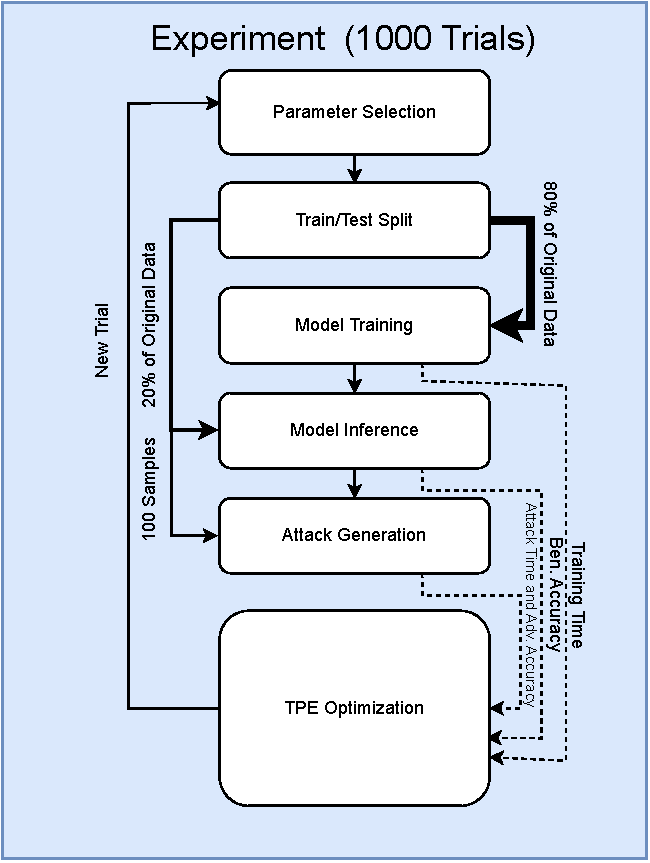
\includegraphics[width=.45\textwidth]{plots/experiment.pdf}
    \caption{Experimental Pipeline Diagram}
    \label{fig:experiments}
\end{figure}



\subsection{Accuracy}
\label{acc}
 It measures the vulnerability or susceptibility of the model to noise-induced failures. A higher failure rate indicates a higher rate of misclassifications or incorrect predictions, signifying a weaker model in terms of \textit{robustness} against noise-induced failures. Throughout, we use the terminology \textit{benign accuracy} to refer to the performance on the test set using unperturbed data. The benign accuracy, $\lambda_{ben}$, is defined as
\begin{equation}
    \lambda:= \mathrm{Accuracy} := 1 - \frac{\mathrm{False~Classifications}}{\mathrm{Total~Classifciations}},
    \label{eq:acc}
\end{equation}
which is generally assumed to indicate the rate of failures in real-world data drawn from the same distribution as the test data~\cite{tan2021critical}. However, the normal test/train split methodology consistently overestimates the model's performance in the presence of adversarial noise~\cite{croce_reliable_2020}. In addition, it ignores the run-time cost of a given architectural decision, caring only for marginal accuracy gains on benchmark data~\cite{desislavov2021compute,bailly2022effects}. Additionally, it has been shown that it is trivial to generate adversarial counter examples that reveal the test/train split methodology to be optimistic at best~\cite{carlini_towards_2017,adversarialpatch,pixelattack,hopskipjump,biggio_poisoning_2013,chakraborty_adversarial_2018,dohmatob_generalized_2019,meyers}. \cm{We use $\lambda_{ben}$ to denote the accuracy on the unperturbed test set $\lambda_{adv}$ to denote the accuracy on the adversarial examples.}

\subsection{Failure Rate}
\label{failure_rate}
The failure rate, denoted by $h$, refers to the percentage or proportion of examples that cause the targeted ML model to misclassify or produce incorrect outputs \cite{meyers}. To encompass the cost of a particular model or attack, the proposed methodology considers failures to be a function over some time interval (\textit{e.g.}, training time, inference time, attack generation time, \textit{etc.}) and some covariates, $\theta$, \cm{such that the failure rate is}
\[
    h_{ \theta}(t) :=  \frac{\mathbb{P}(\textrm{False~Classification})}{\Delta t} t,
\]
where $\mathbb{P}(\textrm{False~Classification})$ is the probability of a false classification, $\Delta t$ is a time interval, and $t$ is a point in time. \cm{Note that  $1 - \text{Accuracy}$  is an estimate of this value when $\Delta t = t$ and converges to this value as the number of samples, $N \rightarrow \infty$. By reparameterizing accuracy as a function of time, one can model the cost (measured in time) to performance (indicated by the number of failures) ratio with an accelerated failure rate model.}


\subsection{AFR Models}
\label{survival_time}
\cm{Accelerated failure rate models are widely used in industrial, medical, or risk-mitigation contexts \cite{kleinbaum1996survival, aft_models} to model the effect of covariates on a model's expected time-to-failure (also called survival time or $S_{\theta}(t)$. For industrial components, this often means testing the component under a variety  of extreme circumstances to induce failures prematurely. For medical applications, this is used to model the effect of demographic characteristics or the efficacy of certain treatments on a given disease. For machine learning, this means inducing failures during training to measure generalization performance.} 

The point of this is to model the \textit{survival time}, $S_{\theta}(t)$, as a function of the time, $t$,  and some set of model parameters, $\theta$ such that,
$$
S_{\theta}(t)= \mathbb{P}(T>t) = \exp\left(-\int_0^t h_{\theta}(u) \, du\right)
$$
\cm{where $\mathbb{P}(T>t)$ is the probability that a model has not failed by time $t$. Then, the expected survival time is}
\[
	\mathbb{E}_{S_\theta}[T] = \int_0^{\infty}  S_\theta(t) \,dt.
\]

However, modelling $S_{\theta}(t)$ requires a choice in modelling function for $S_{\theta}$. The Log-Logistic, Log-Normal, and Weibull functions are widely used alternatives~\cite{kleinbaum1996survival}.  \cm{For each trial, one can measure the inference time to define the time interval and the accuracy to estimate the number of failures in that time interval. This should be measured in both the benign and adversarial contexts as a way to measure the cost of a particular model in both contexts.}

To choose a best-fit from the possible AFR functions, one should compare Akaike Information Criterion (AIC), Bayesian Information Criteria (BIC), and Concordance following the best-practices of this methodology~\cite{aft_models,kleinbaum1996survival}. \cm{For AIC and BIC, that means choosing the smallest value. Concordance, however, is a number between $0$ and $1$ that quantifies the degree to which the survival time is explained by the model, where a $1$ reflects a perfect explanation~\cite{kleinbaum1996survival} and .5 reflects random chance. By evaluating $\mathbb{E}_{S_\theta}[T]$ for both adversarial and benign data, we can test the model under extreme perturbations and minimize the number of evaluated samples~\cite{aft_models,kleinbaum1996survival} rather than relying on the $> 10^{12}$ samples as required by ISO26262~\cite{iso26262}}


\subsection{Benign and Adversarial Survival Time}
\label{accelerated}
Using accelerated failure rate models, we can find the expected survival time under optimistic circumstances, $S_{ben}$ as well as under adverse ones (accelerated failure rate), $S_{adv}$. The survival time for benign samples is
$$
    S_{ben} := S(t_i; x, y, \theta) \mathrm{~~where~~} \varepsilon = 0
$$
and the survival time for the adversarial samples is
$$
    S_{adv} :=  S(t_i; x, y, \theta) \mathrm{~~where~~} 0 < \varepsilon \leq \varepsilon_{max}.
$$
\cm{This can also be thought of in terms of the accelerated failure rate assumption~\cite{kleinbaum1996survival}:
\begin{equation}
S_{adv} \approx  \phi S_{ben}(\phi t)
\label{assumption}
\end{equation}
where $\phi$ is some acceleration factor describing the joint effect of the covariates. This assumption means we can evaluate the benign accuracy using a small number of adversarial samples ~\cite{kleinbaum1996survival}, with our precision coming from careful time measurements rather than massive test sets.} 
\cm{However, in order to find the optimal hyper-parameter configurations for both the model and attack, one must search this space intelligently.}


\subsection{Optimisation}
\label{optimisation}
\cm{Machine learning models are typically trained across a wide variety of hyper-parameters to determine the ``best" model by minimizing an optimisation program (minimizing a loss function associated with the machine learning problem) by measuring the loss across many configurations of a model.} However, the number of hyper-parameter combinations are often infinite or at least exponential in the number of such parameters,
making it infeasible to exhaustively evaluate the search space. Additionally, the goals of test-set accuracy and adversarial accuracy are often at odds~\cite{carlini_towards_2017}--with several researchers noting an inverse relationship between model accuracy and model robustness ~\cite{carlini_towards_2017,meyers}. Therefore, a proper search would keep this dual-objective in mind.
\cm{To optimize for adversarial and benign accuracy simultaneously, we propose the use of the Tree-structure Parzen Estimator (TPE) while converging  over tens or hundreds of trials~\cite{ozaki2020multiobjective}}.







\subsection{Advantages of this Methodology}
\label{advantages}
\cm{Because of the small number of samples needed for building AFR models (when compared to testing against massive in-distribution test sets), AFR models could}, for example, act as a unit test in machine learning applications rather than relying on full-system integration tests to evaluate changes to a single model, signal processing technique, data storage format, or API access mechanism~\cite{schmoor2000sample,lachin1981introduction}. It could also be used to highlight error-prone classes or other subsets of data to reduce error or create synthetic samples as is common in medical research~\cite{kleinbaum1996survival}. Furthermore, by isolating changes and testing them as quickly as possible, it is  easier to parse cause and effect when compared to full-system integration tests that could include many changes from many different development teams and require live and potentially dangerous systems (like cars or MRI machines) to effectively test. To further increase development velocity, these models can quantify the marginal risk associated with each change, as dictated by the ISO 26262 standard \cite{iso26262}. This risk analysis is outlined in the subsection below.

\section{Cost Analysis}
\label{cost}
\cm{In addition to the survival analysis, we can use an estimate of survival time to conduct a cost analysis as dictated by ISO26262~\cite{iso26262} which allows us to quantify the marginal risk. To quantify this marginal risk, one must measure} the benign and adversarial accuracies (see Eqs.~\ref{eq:adv_success}~and~~\ref{eq:acc}), the model training time ($t_{t}$), the model inference time or latency ($t_{i}$), the attack generation time ($t_{a}$), the cost per hour for a particular hardware ($C$), as well as the power consumption ($P$) of each tested model and attack. The final subsection outlines why these metrics are important and their usage in this methodology.

\subsection{Accuracy}
\cm{In order to estimate the number of failures in a given time period}, we measured both the benign accuracy and the adversarial accuracy, which reflect the normal test-set accuracy and the test-set accuracy in the presence of additive noise in the direction that maximizes loss. \cm{Under the AFR framework above, we can use the adversarial accuracy as a measure of the survival time across a specified time period.}


\subsection{Training Time}
The training time, $T_t$, is the time it takes to evaluate $n$ samples such that the training time per sample $t_t$ is
$$
    T_t := t_t * n  * m.
$$
where $m$ is the number of epochs and $*$ is normal scalar multiplication.

\subsection{Latency}
Latency is the time it takes to respond to a query. We assume that latency per sample is
$$
    T_i := t_i *n,
$$
which will be driven by the memory bandwidth (measured in bits/second) of a given CPU or GPU and the size\cite{vgg} and complexity\cite{resnet} of a given neural network architecture.


\subsection{Attack Generation Time}
A successful attack is one that induces failure in a model. That is, the expected survival time, $\mathbb{E}_{S_\theta}[T]$, can be thought of as the average time it takes for an attacker to induce a change in the model output. We approximate this for each attack/defence configuration by the total attack time, $T_a$, for $n$ samples, $i$ iterations, and attack time per sample, $t_a$, as
\begin{equation}
    \label{attack_time}
    T_a := t_i *n *i.
\end{equation}
We restricted this to a single iteration \cm{such that $i =1$} as described in FGM~\cite{fgm}.


\subsection{Cost}
Furthermore, we approach the cost of deployment at two scales. Firstly, we consider the cloud-rental scale, where a small-business might test and deploy a model, using Google Cloud Platform\footnote{\href{https://cloud.google.com}{https://cloud.google.com}} (GCP) compute costs as a measure of total cost. However, at a certain scale, (\textit{e.g.} for deploying a self-driving car) it is  more appropriate to talk about cost in terms of power. Finally, we define best-case and worst-case success metrics that provide an efficient way to minimize the latency, cost of deployment, and 
maximize the generalized performance of a model. We define the training cost ($C_t$) as
$$
    C_t = C_h *T_t,
    \label{eq:cost_training}
$$
the cost of model inference time as,
$$
    C_i = C_h *T_i,
    \label{eq:cost_inference}
$$
and the cost of an attack as,
$$
    C_a = C_h * T_a.
    \label{eq:cost_attack}
$$
where $C_h$ is the cost per unit time for the hardware, $T_t$ is the training time, $T_i$ is the inference time, and $T_a$ is the attack generation time.

\subsubsection{Power}
The power consumption for a particular piece of hardware ($P_h$), measured in Watts (Joules per second), can be thought of similarly such that the total power consumption of model training is
$$
    P_t = P_h *T_t,
    \label{eq:power_training}
$$
the power consumption during model inference is
$$
    P_i = P_h *T_i,
    \label{eq:power_inference}
$$
and the power consumption during attack generation is
$$
    P_a = P_h *T_a.
    \label{eq:power_attack}
$$
where $P_h$ is the cost per unit time for the hardware, $T_t$ is the training time, $T_i$ is the inference time, and $T_a$ is the attack generation time.

\subsection{Comparative Risk}
\cm{One advantage of this survival analysis is that we can directly compare the marginal risk and reward for a particular model choice. The \textit{marginal risk} is the change in survival time divided by change in attack compared to some control model such that:
\[
    \textrm{Comparative~Risk} := \frac{\% \Delta S(t)}{\% \Delta C_a},
\]
where $\% \Delta$ reflects the percent change from the control model.}

\cm{Another advantage is that we can quickly discard ineffective model choices with this method.} In security analysis, it is  routine to think in optimistic terms for both the attacker and defender. \cm{In cryptography, these ideal attack- and defence-scenarios are used to test the computational feasibility of subverting a particular cryptographic system~\cite{kamal2017study,leurent2020sha} (\textit{e.g.}, whether or not a given cryptographic method should be considered ``broken"). For our purposes, by assuming the best-case scenario for both attacker and defender, we can model the Pareto front --- the best-case asymptotic behavior --- of either party~\cite{zitzler2008quality}.}
As such, we center our analysis on the Fast Gradient Method~\cite{fgm} (see: Eq.~\ref{eq:fgm}) which is both effective and fast~\cite{meyers}. If the cost to a model builder is much larger than the cost to an attacker ($C_t \gg C_a$), then it is  clear that the model is ``broken" in this cryptographic sense and can be discarded as ineffective. 





\section{Experiments}
\label{experiments}

This section outlines specific implementation details for the evaluation of the methodology outlined in Section~\ref{afr}.


\subsection{Cloud Platform and Hardware}
To conduct the experiments and have access to different types of hardware, we utilized GCP. Six virtual machines running Container Optimized Operating System provided by GCP constituted our testbed. Using Google Kubernetes Engine 1.27.3 and Containerd 1.7.0,  we created a cluster consisting of six worker nodes. Three worker nodes were responsible for running the monitoring platforms such as Prometheus 2.47.2 and Grafana 10.2.0. These nodes were of the ``e2-medium" instance type provided by GCP. In total, we used three GPU models. For P100 and V100 GPUs, we used ``n1-standard-2'' type for the nodes and for L4 GPUs we used ``g2-standard-4''.

To assess the energy consumption of the experiments deployed on a Google Kubernetes Engine, we employed Kubernetes Efficient Power Level Exporter (KEPLER) as our measurement tool~\cite{amaral2023kepler}. This approach enables us to gather energy consumption data on granular level as it runs in Kubernetes cluster and capable of collecting energy consumption of Kubernetes components. In essence, KEPLER uses extended Berkley Packet Filter (eBPF) to probe energy-related system stats and exports them as Prometheus metrics. eBPF can be described as a lightweight and sandboxed virtual machine (VM) in kernel space. eBPF programs are invoked by the kernel when certain events occur. Examples of such events include system calls or network activity. These processes enable deep analysis and full control over different events with low overhead~\cite{sedghpour@ebpf}. A diagram of the cloud architecture can be found in Fig.~\ref{fig:architecture}. Finally, to meet our goal of developing a cost-effective model evaluation technique, we restricted all of the experiments to a single one-thousand United States dollar research grant from Google. Approximately 10\% of this was used for development and 90\% was used for the evaluations.

\begin{figure*}
    \centering
    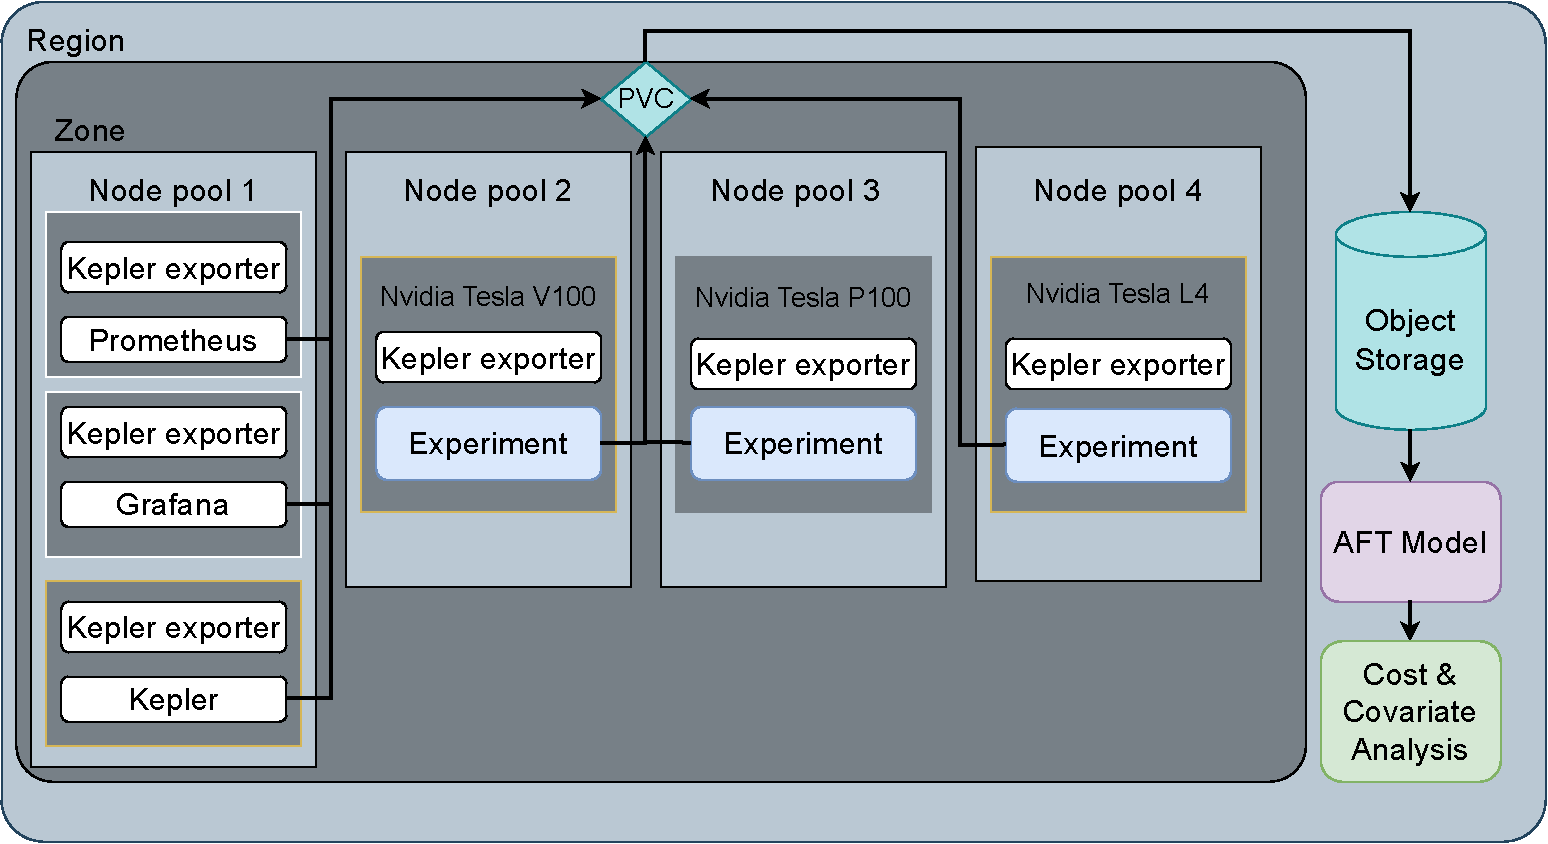
\includegraphics[width=.8\textwidth]{plots/architecture.pdf}
    \caption{Cloud Architecture Diagram}
    \label{fig:architecture}
\end{figure*}


\subsection{AFR Models}

For each hardware configuration and dataset, we ran one thousand trials, a number that should converge to a Pareto-optimal result~\cite{ozaki2020multiobjective,zitzler2008quality} for the TPE algorithm, within some expected error bounds ~\cite{legriel2010approximating}. We used three optimisation criteria-- benign accuracy, training time, and adversarial accuracy seeking to maximize both benign and adversarial accuracy while minimizing training time (and therefore deployment cost). We selected a set of parameters as per the TPE algorithm and trained on 80\% of the samples. Of the remaining samples, 100 were withheld to be attacked and used to evaluate the adversarial accuracy. Fig.~\ref{fig:experiments} illustrates this methodology. For each dataset, we tested this on ten random splits of the data. For each trial, we recorded attack generation time, model training time, model inference time, benign accuracy and adversarial accuracy, and the size of the training set, test set, and attack. Using these values, we fit an AFR model to the number of failures (indicated by accuracy and sample size) and the attack generation time. The inference time and training time were used to conduct the cost analysis outlined in the next section (Sec.~\ref{cost})

\subsection{Datasets}
The AFR models were evaluated using the MNIST~\cite{mnist}, CIFAR10\cite{cifar}, and CIFAR100\cite{cifar} datasets, chosen primarily for their standardized use in adversarial analysis~\cite{madry2017towards,croce_reliable_2020,carlini_towards_2017,deepfool} and decades of experimental results.
Before training, we centered and scaled the data so that the attack distance would be analogous for all tested datasets. Furthermore, to reduce the complexities of system overhead, distributed or federated training, and the effect of shared cloud environments, we restricted ourselves to datasets that were small enough to reside entirely within GPU memory with the model, since the disk read speed in cloud environments is incredibly variable.


\subsection{Models}
We restricted ourselves to a single model for our evaluations. Primarily, this was done to meet the budgetary constraints since evaluating more models would mean evaluating fewer pieces of hardware. As discussed in Sec.~\ref{learning_rate}, the relationship between hardware specifications, model-size, data distribution, the optimal learning rate, the optimal batch size, and the optimal number of epochs is highly complex and hard to predict. So, we sampled learning rates $\in [10^{-6}, 1]$, batch sizes $\in [1, 10^5]$, and epochs $\in [1, 50]$ for MNIST and CIFAR10 on the P100 and V100. For CIFAR100, we increased the range of the tested epochs to be $\in [1, 100]$. To evaluate the efficacy of different bit-depths on the L4 hardware, we used the Feature Squeezing defence~\cite{feature_squeezing} provided by IBM's adversarial robustness toolbox~\cite{art2018} with bit depths $\in [4,8,16,32,64]$ which casts the inputs into \texttt{Pytorch} compatible arrays. Model parameters were chosen using the \texttt{Optuna} optimisation framework, the configuration was handled by \texttt{hydra}, and \texttt{dvc} was used to ensure reproducibility and aid in collaborative development.


\subsection{Attacks}
Since one goal of this paper was to evaluate how hardware and deployment cost affect adversarial robustness during run-time, we focused on evasion attacks since they induce failures by adding noise to the data at run-time. Prior research~\cite{meyers} has shown that the Fast Gradient method (see Eq.~\ref{eq:fgm}) is consistently the most effective at inducing a large number of failures in a small amount of time. To evaluate the effect of adversarial noise on our samples, we varied $\varepsilon \in [0, 1]$, using the \texttt{adversarial-robustness-toolbox} package maintained by a team at IBM~\cite{art2018}.


\subsection{GPU Configurations}
We tested several hardware configurations, which have various hourly costs, peak power demands, and theoretical memory bandwidths. The V100 was chosen as a baseline, since it is  routinely used in the literature ~\cite{svedin2021benchmarking,xu2018deep}. The P100 architecture comes from the same line of server-grade GPUs, but from an older generation. The L4, however, is advertised as a machine built for inference --- not training --- relying on a smaller number of bits per tensor core. Consequently, the number of operations per second is dependent on the bit depth of the data and the model weights, with the peak numbers outlined in Tab.~\ref{tab:hardware} referring to 8-bit inputs.

\begin{table}[h]
    \centering
    \begin{tabular}{lllll}
    \toprule
                            & V100   & P100   & L4    &  \\
    \midrule
    Cost (USD/hour)         & 2.55   & 1.60   & 0.81   &  \\
    Power (Watts)           & 250    & 250    & 72    &  \\
    Memory Bandwidth (GB/s) & 900    & 732    & 300   &  \\
    \bottomrule
    \end{tabular}
    \caption{Hardware specifications for tested GPUs. All specifications were retrieved from the Nvidia website at the following links: 
    \href{https://images.nvidia.com/content/technologies/volta/pdf/volta-v100-datasheet-update-us-1165301-r5.pdf}{V100 Datasheet},
    \href{https://images.nvidia.com/content/tesla/pdf/nvidia-tesla-p100-PCIe-datasheet.pdf}{P100 Datasheet}, and
    \href{https://nvdam.widen.net/s/rvq98gbwsw/l4-datasheet-2595652}{L4 Datasheet}. Prices were retrieved from Google Cloud Platform for the \texttt{europe-west4} region on 3 December 2023 at \href{https://cloud.google.com/pricing/list}{this link.}
    }
    \label{tab:hardware}
\end{table}

\subsection{Survival Analysis}
In addition to the optimisation criteria of benign/adversarial accuracy and training time, we collected prediction times, attack times, power consumption, batch size and number of epochs to be used as covariates of the funciton, $S(t)$. We attempted adding dummy variables for hardware (\textit{e.g.}, peak power and peak bandwidth) as well as the datasets (\textit{e.g.}, resolution, bit depth, and number of color channels), but each of these were strongly co-linear with training time and hindered modelling. As such, they were not included. To fit the AFR model and to plot the effect of covariates, we used the \texttt{lifelines} Python package~\cite{lifelines}. We also compared the chosen modelling functions (see Section~\ref{afr}).  These results can be found in Section~\ref{results}.



\subsubsection{Hardware}
The rental cost of the hardware, measured in United States Dollars per hour, will indicate the operating cost of a given model. To calculate this, we used the price per hour from each of cloud service pricing page\footnote{Google Cloud prices for P100 and V100 obtained \href{https://cloud.google.com/compute/gpus-pricing}{here.}}\footnote{Google Cloud prices for L4 obtained  \href{https://cloud.google.com/compute/vm-instance-pricing\#accelerator-optimized}{here.}} and calculated the cost of training ($C_{t}$) and the ($C_{i}$) from the cost of hardware ($C_{h}$), the training time ($T_{t}$), and the inference time ($T_{i}$).





\section{Results and Discussion}
\label{results}

Below, we demonstrate the effect of hardware and dataset on the benign/adversarial accuracy (Fig.~\ref{fig:acc}), training/inference/attack time (Fig.~\ref{fig:time}), and both monetary (Fig.~\ref{fig:cost}) and power (Fig.~\ref{fig:power}) costs for training/inference/attacks. We also compared all three survival times outlined in Sec.~\ref{afr} using the criteria outlined in the same section. Using the best-fit function (again, see Sec.~\ref{afr}), we examined the effect of the covariates on the survival time of the model (Figs.~\ref{fig:partial_effect_train_time}-\ref{fig:partial_effect_attack_eps}).

\cm{I will cut this accuracy subsection. In exchange, I will conduct a log-rank test}
\subsection{Accuracy}
Fig.~\ref{fig:acc} shows the advernsarial and benign accuracies for all datasets and hardware. It demonstrates little to no change in accuracy or adversarial accuracy, regardless of hardware though CIFAR10 has worse benign performance and CIFAR100 has substantially worse adversarial performance. For all three datasets, the adversarial accuracy becomes the reciprocal of the number of classes (e.g. the accuracy we would expect on random noise), demonstrating the efficacy of the attack outlined in Sec.~\ref{optimisation}.

\begin{figure}[h!]
    \centering
    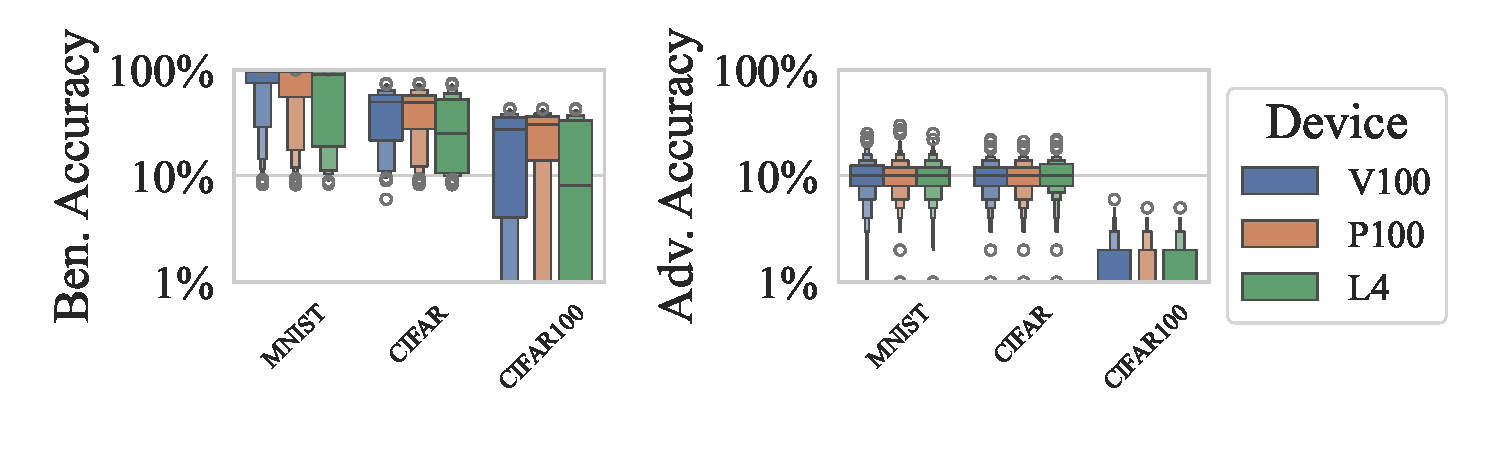
\includegraphics[width=0.5\textwidth,trim={30pt 0 10pt 0},clip]{plots/combined/acc.pdf}
    \caption{Ben. and Adv. Accuracy Across Datasets and Hardware}
    \label{fig:acc}
\end{figure}


\subsection{Time}
Fig.~\ref{fig:time} reveals the training time. Slower hardware (see Memory Bandwidth in Tab.~\ref{tab:hardware}) is only a few milliseconds slower, so this is unlikely to be noticeable to an end-user during inference. This should be no surprise since the less-capable hardware is meant to be used exclusively for inference. Additionally, the attack time increases with both the training and prediction times across hardware and datasets --- an expected result since this is driven by the number of samples and the inference time (see Eq.~\ref{attack_time}).

\begin{figure}[h!]
    \centering
    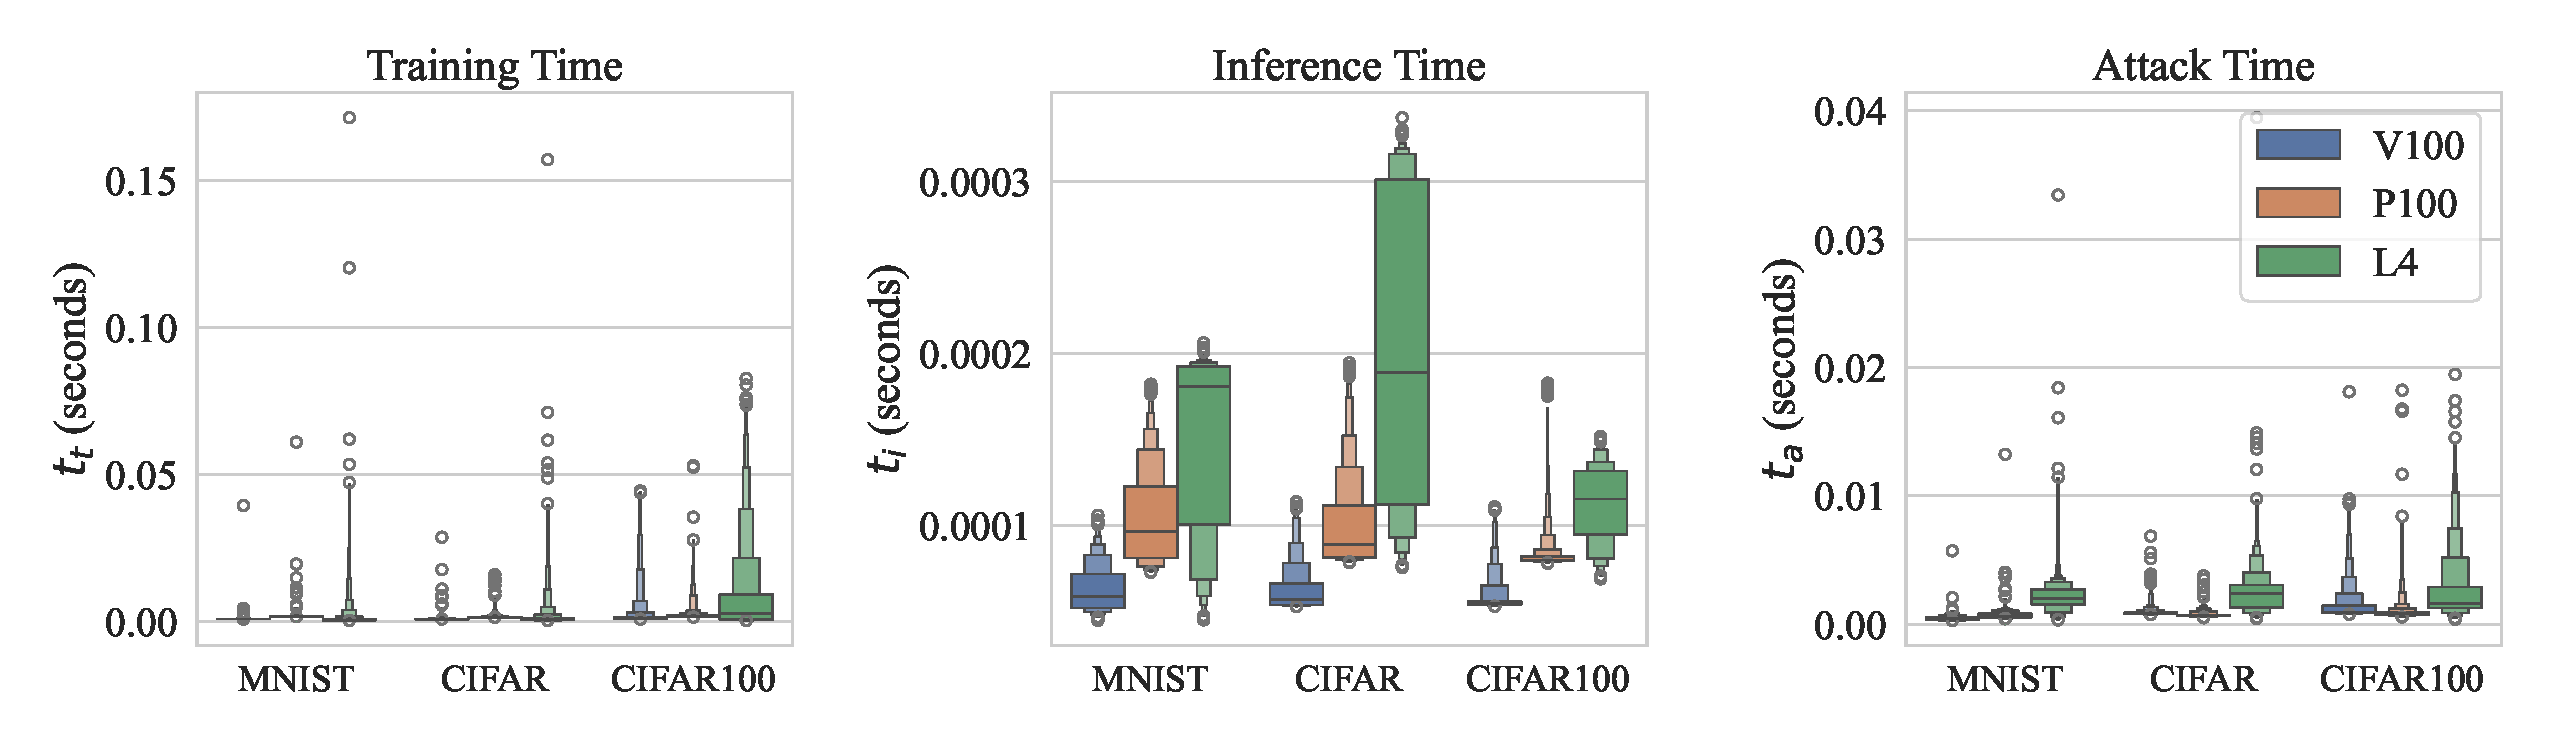
\includegraphics[width=0.5\textwidth,trim={100pt 0 100pt 0},clip]{plots/combined/time.pdf}
    \caption{Training, Prediction, and Attack times across datasets and hardware.}
    \label{fig:time}
\end{figure}


\subsection{Power}
The power consumption, illustrated in Fig.~\ref{fig:power}, tracks monetary cost (Fig.~\ref{fig:cost}) closely, probably because that's the predominant cost for the datacenter itself~\cite{dayarathna2015data}, so it is unsurprising that cloud billing is colinear with this metric. Furthermore, we see that the largest dataset (CIFAR100) and smallest GPU (L4) require the least amount of power (Fig.~\ref{fig:power}). 

\begin{figure}[h!]
    \centering
    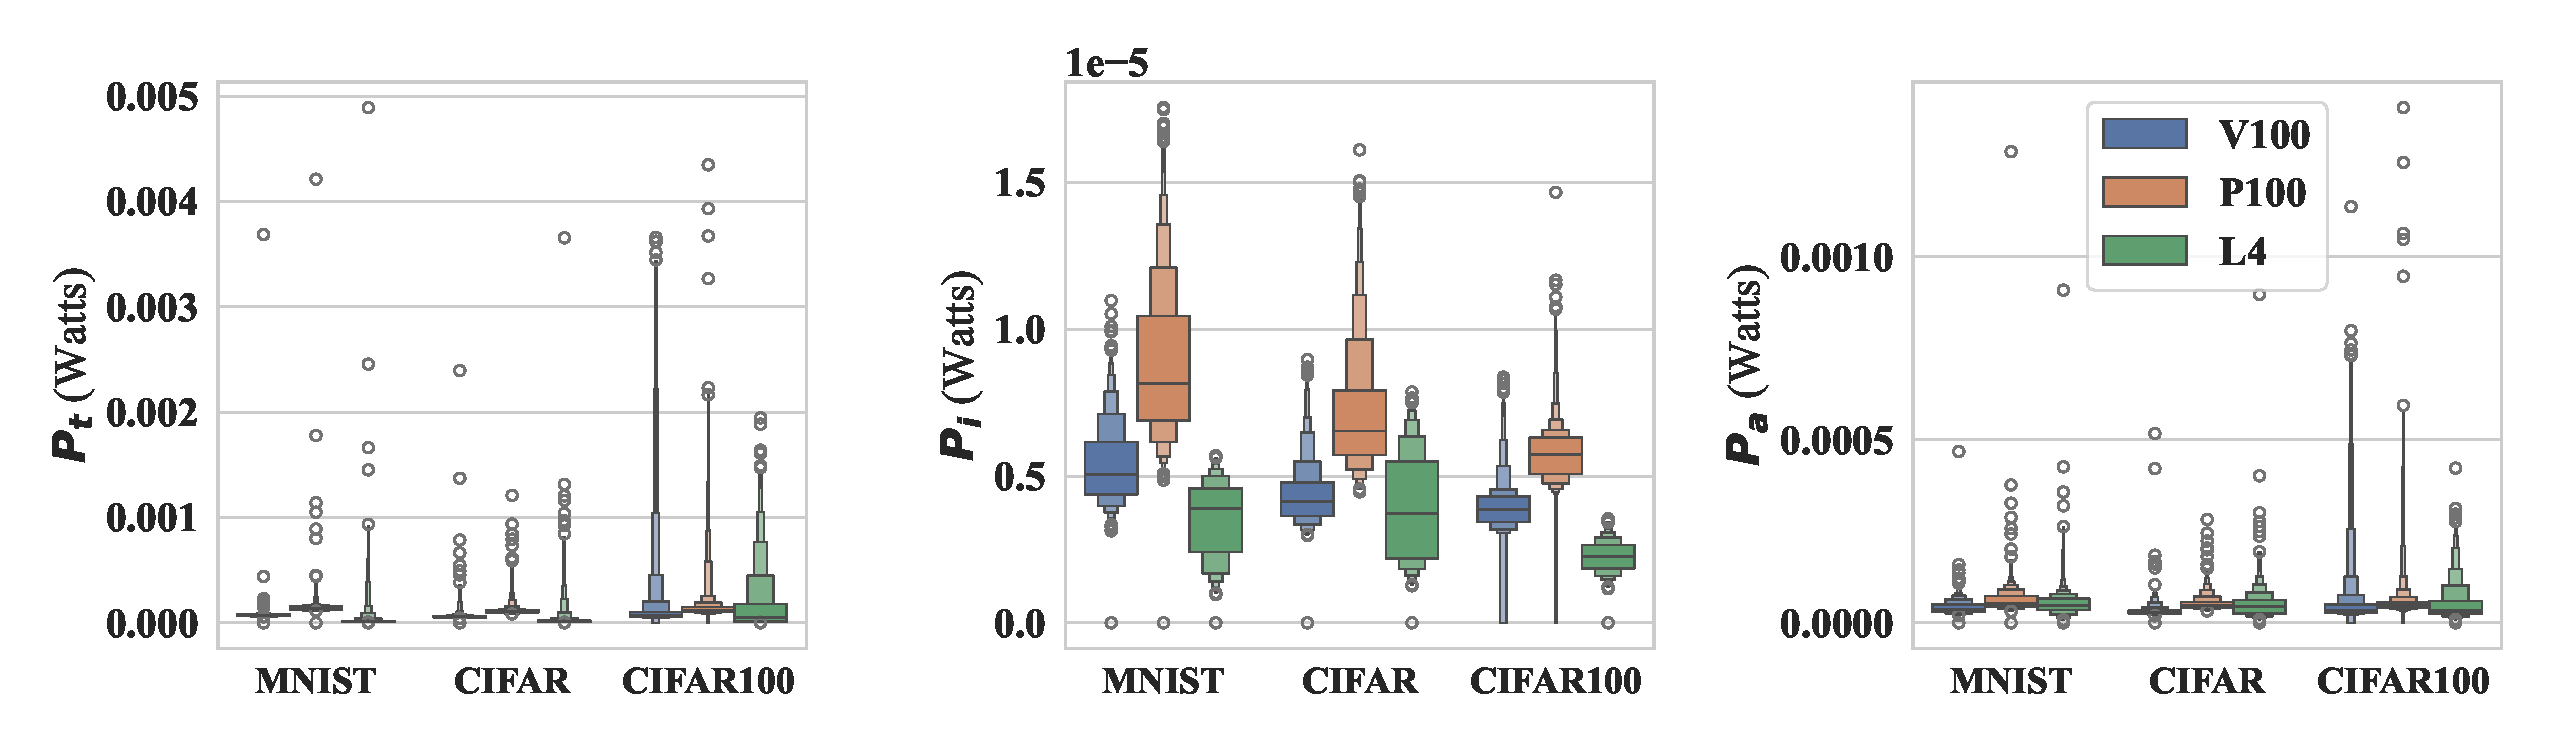
\includegraphics[width=0.5\textwidth,trim={100pt 0 100pt 0},clip]{plots/combined/power.pdf}
    \caption{Training, Prediction, and Attack Power Consumption Across Datasets and Hardware}
    \label{fig:power}
\end{figure}


\subsection{Cost}
The monetary cost for each dataset and each piece of hardware is shown in Fig.~\ref{fig:cost}. \cm{For all three datasets across all three pieces of hardware, the cost of training on a single sample often exceeds the cost of attacking a single sample. In the best case scenario, they are comparable. However, we note that the attacker only needs to be lucky once, whereas the the model builder must be lucky always. This reveals an essential advantage for the attacker on the reference model and hardware architecture --- attacks consistently succeed with 100s of samples while model training requires orders of magnitude more.}

\begin{figure}
    \centering
    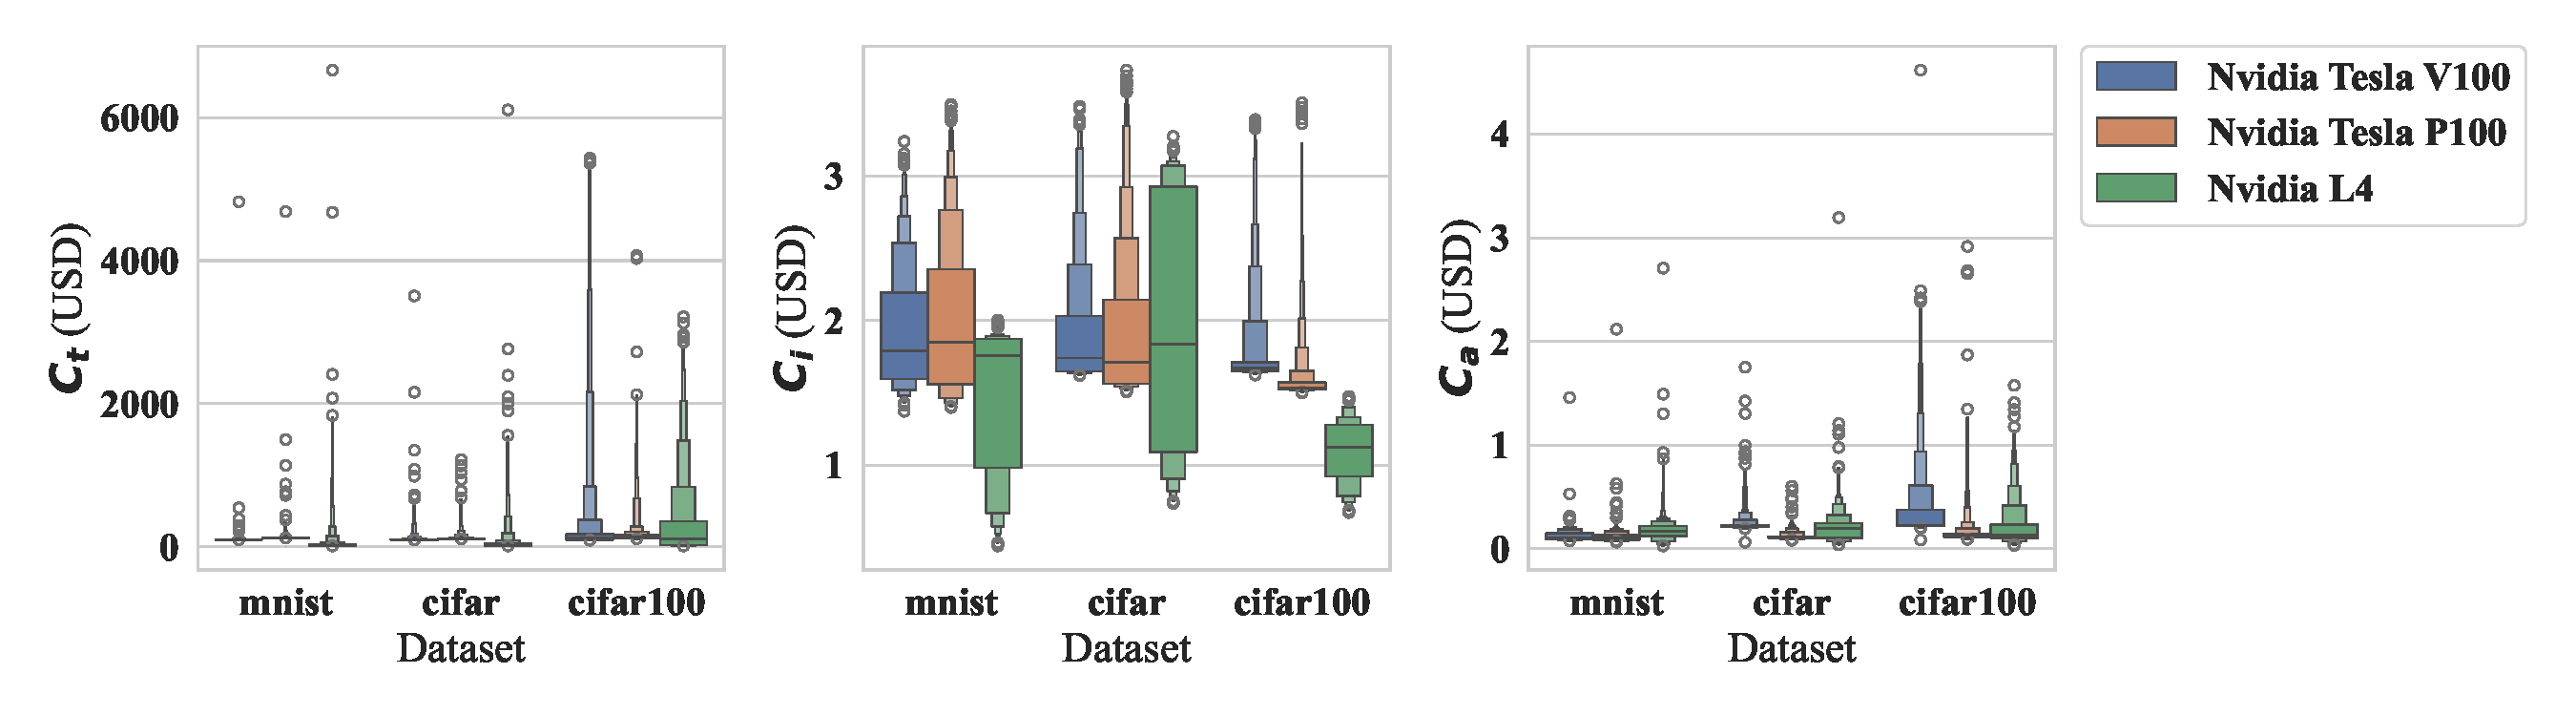
\includegraphics[width=0.5\textwidth,trim={100pt 0 100pt 0},clip]{plots/combined/cost.pdf}
    \caption{Training, Prediction, and Attack Monetary Cost Across Datasets and Hardware}
    \label{fig:cost}
\end{figure}



\subsection{AFR Models}
\cm{TODO: add 1. fitted parameters and 2. their statistical significance here. Discuss what that means. Move table here. Discuss why we chose Log-Logistic. Discuss accelerated failure assumption again.}

Table~\ref{tab:Combined} shows that the aft models using log-logistic and log-normal functions have similar predictive abilities, but we used the log-logistic model to render the plots due to its marginally improved AIC.

\begin{table*}
\centering
\caption{Comparison of AFR Models on the Combined dataset. The metrics are defined in Sec.~\ref{afr}}
\label{tab:combined}
\begin{tabular}{lrrrrrr}
\toprule
 & AIC & BIC & Concordance & Test Concordance & ICI & E50 \\
\midrule
Weibull & -5.57e+03 & -5.57e+03 & 0.84 & 0.84 & 0 & 0 \\
Log Logistic & -5.71e+03 & -5.71e+03 & 0.85 & 0.84 & 0.01 & 0 \\
Log Normal & -5.85e+03 & -5.85e+03 & 0.84 & 0.84 & 0.01 & 0 \\
\bottomrule
\end{tabular}
\end{table*}


\cm{Figure TODO shows the p-values for each of the covariates}

Figure~\ref{fig:partial_effect_train_time} shows that training time, by itself, does little to influence the model's survival time. However, as we see in Fig.~\ref{fig:partial_effect_attack_eps}, that and increasing the attack distance ($\varepsilon$) by an order of magnitude only marginally reduces the survival time. Additionally, that the benign accuracy, Fig.~\ref{fig:partial_effect_accuracy}, is an equally poor indicator of adversarial robustness, raising further concerns about the efficacy of the train/test split methodology.

% \begin{figure}
%   \centering
%   % include first image
%   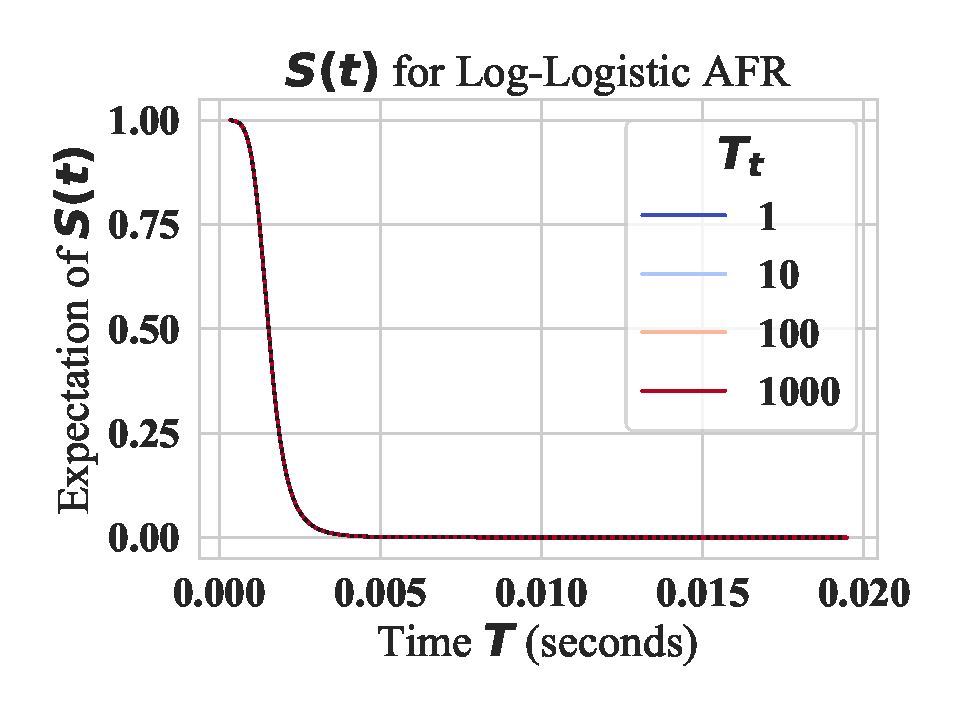
\includegraphics[width=0.8\linewidth,trim={20pt 20pt 20pt 20pt},clip]{plots/combined/log_logistic_train_time_partial_effect.pdf}  
%   \caption{The partial effect of the training time on the survival time across all datasets and models according to the function $S(t)$ as outlined in Section~\ref{survival_time}. The dotted line represents the baseline survival function $S_{ben}$.}
%   \label{fig:partial_effect_train_time}
% \end{figure}

\begin{figure}
  \centering
  % include second image
  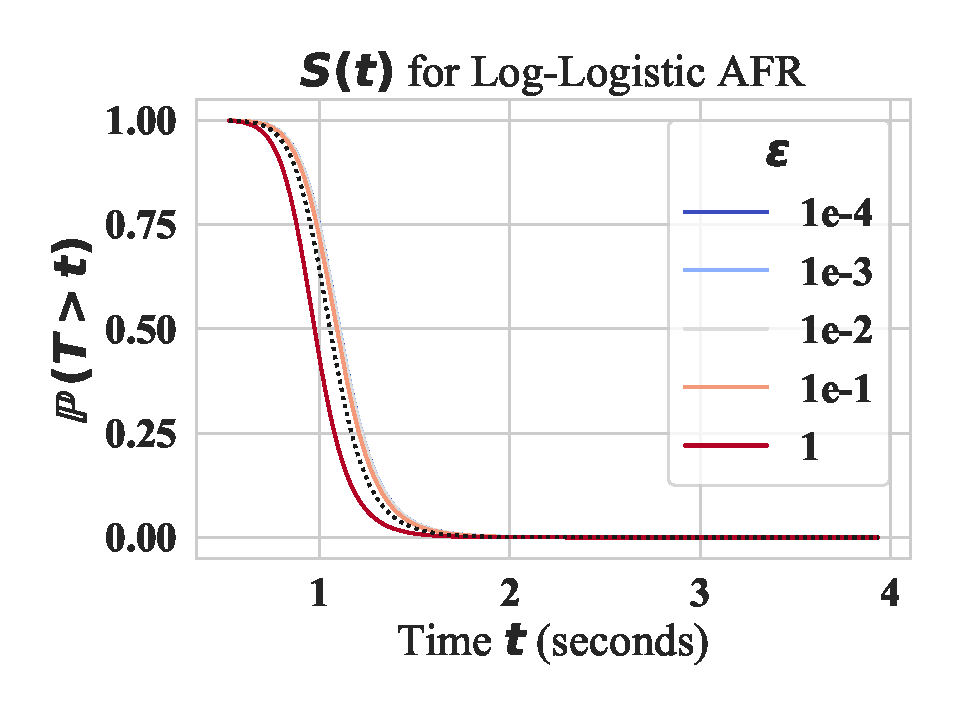
\includegraphics[width=0.8\linewidth,trim={20pt 20pt 20pt 20pt},clip]{plots/combined/log_logistic_attack_eps_partial_effect.pdf}  
  \caption{The partial effect of the attack distance on the survival time across all datasets and models according to the function $S(t)$ as outlined in Section~\ref{survival_time}. The dotted line represents the baseline survival function $S_{ben}$.}
  \label{fig:partial_effect_attack_eps}
\end{figure}

\begin{figure}
  \centering
  % include second image
  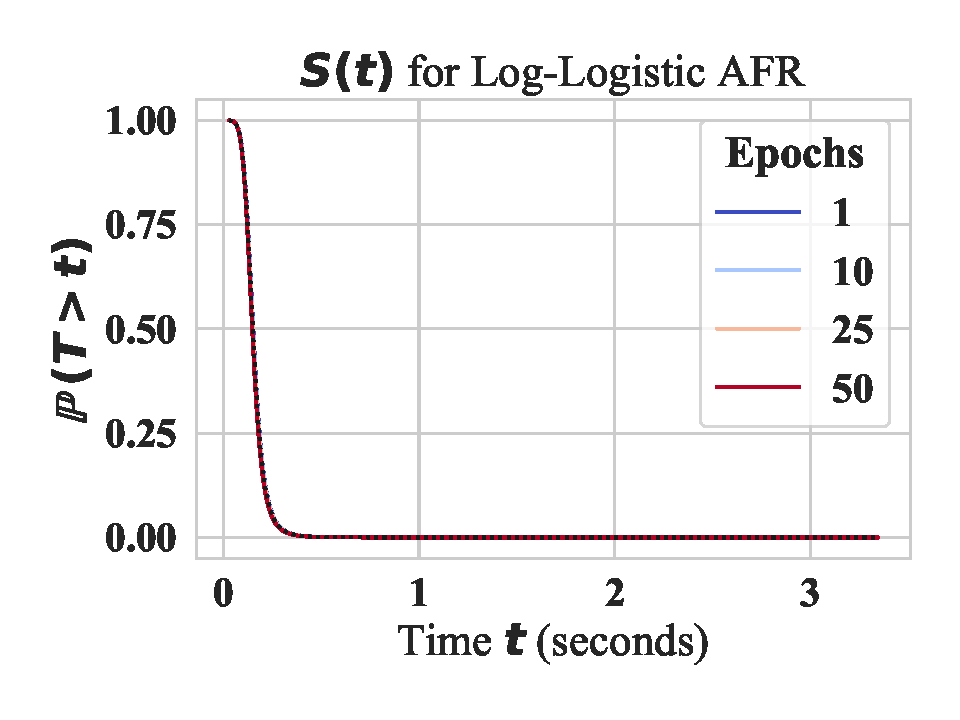
\includegraphics[width=0.8\linewidth,trim={20pt 20pt 20pt 20pt},clip]{plots/combined/log_logistic_epochs_partial_effect.pdf} 
  \caption{The partial effect of the accuracy on the survival time across all datasets and models according to the function $S(t)$ as outlined in Section~\ref{survival_time}. The dotted line represents the baseline survival function $S_{ben}$.}
  \label{fig:partial_effect_epochs}
\end{figure}

\begin{figure}
  \centering
  % include second image
  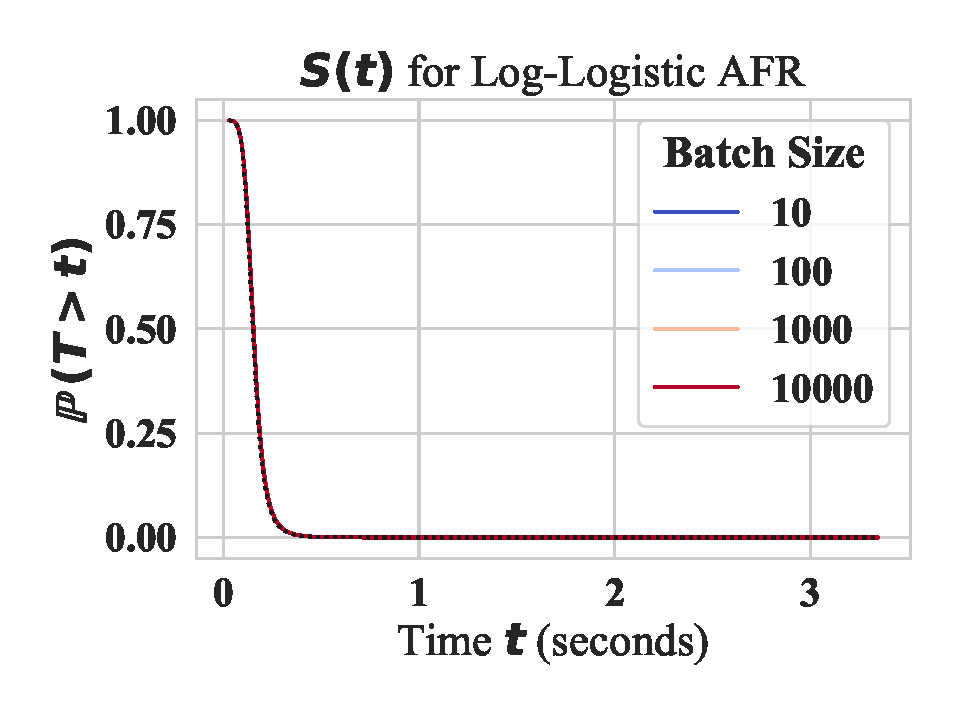
\includegraphics[width=0.8\linewidth,trim={20pt 20pt 20pt 20pt},clip]{plots/combined/log_logistic_batch_size_partial_effect.pdf} 
  \caption{TODO: replace this with epochs and batch size}
  \label{fig:partial_effect_batch_size}
\end{figure}



\subsection{Comparative Risk}
\cm{TODO}
Call back to the comparative risk and the fast rejection mechanism. 





\section{Considerations}
\label{considerations}
We have taken much care to conduct these measurements as carefully as possible. Primarily, to minimize timing jitter and account for GPU parallelization, we assumed that the time-to-failure during the benign and adversarial accuracy measurements was uniform across the samples, but independent and identically distributed data is already a pre-condition for maximum likelihood learning~\cite{ma2022state}. Given the strong ($>0.5$) concordance results and uniformity across AFR functions in Table~\ref{tab:Combined}, this assumption appears to be insignificant, though accounting for the failure rate per sample or class is likely to account for some of the remaining unexplained variance. Additionally, we chose a model and set of datasets small enough to fit entirely in GPU memory to minimize the confounding factors around parallelized, distributed, and/or federated learning. \cm{While this obscures the effect of GPU parallelization, the result doesn't change since all metrics are measured on a particular piece of hardware for both the attacker and defender. Furthermore, we see the attack batch size and the training batch size to be the same for every trial. If anything, the smaller sample size of the attacks means that proportionally more parallelization overhead is needed per sample, leading to an underestimate of the attack efficacy.} In general, distributed/federated models are out of scope, but architectural choices regarding the configuration of such methods could be evaluated using the cost and survival analysis techniques outlined above. Larger models acting on larger datasets are likely to perform better on hardware with a higher GPU bandwidth. However, we would like to note that the ``inference-optimized" Nvidia 4-series GPUs are perfectly capable and affordable training machines. We restricted our search to only a single evasion attack (see Eq.~\ref{eq:fgm}) in the interest of time (and therefore deployment cost), though this analysis would generalize to other evasion, extraction, inversion, or poisoning attacks.





\section{Conclusions}
\label{conclusion}
In this work, we introduced survival analysis to machine learning, developed a method to quickly and efficiently test model parameter choices and to evaluate them in the presence of adversarial noise, allowing us the model performance as a function of tested model parameters. Using this technique, we showed that despite reduced run-times with newer and/or larger hardware, that adversarial robustness is not substantially effected and that the specific choice of attack parameters is far more important than model training time. Furthermore, we demonstrate the un-advertised training capability of the Nvidia L4 GPU which yields substantially similar results when compared to more expensive and power hungry hardware. However, the marginal run-time is substantial, even if it's cost-effective.

% no keywords
% For peer review papers, you can put extra information on the cover
% page as needed:
% \ifCLASSOPTIONpeerreview
% \begin{center} \bfseries EDICS Category: 3-BBND \end{center}
% \fi
%
% For peerreview papers, this IEEEtran command inserts a page break and
% creates the second title. It will be ignored for other modes.
\IEEEpeerreviewmaketitle


\clearpage
\bibliographystyle{IEEEtran}
\bibliography{bibliography}
\end{document}



